\documentclass{article}
\usepackage{graphicx} % Required for inserting images
\usepackage{amsmath}
\usepackage[english,russian]{babel}

\title{Работа 1.1.1\\ 
	Определение систематических и случайных погрешностей при измерении удельного сопротивления нихромовой проволоки}


\begin{document}
	
	\maketitle
	
	\section{Аннотация}
	В работе измеряется удельное сопротивление нихромовой проволоки двумя способами: 1) путем анализа графика ВАХ проволоки, 2) путем вычисления по известной формуле \(R = \rho \frac{l}{S}\), где \( R\) измерено  посредством моста Уильсона (моста постоянного тока).\\\\
	\emph{Цель работы:} измерить удельное соединение нихромовой проволоки и вычислить систематические и случайные погрешности при использовании измерительных прибров. \\\\
	\emph{Оборудование:} линейка, штангенциркуль, микрометр, нихромовая проволока, амперметр, стрелочный вольтметр, источник ЭДС, мост Уильсона (мост постоянного тока), реостат, ключ, провода.
	
	\section{Теоритические сведения}
	
	Удельное сопротивление цилиндрической проволоки определяется по формуле:
	\(\rho = \frac{R}{l}S\), а учитывая что S = {\pi}{\frac{d^2}{4}},
	
	$$\rho = \frac{R}{l}{\frac{{\pi}d^2}{4}}$$
	Где $R$ - сопротивление отрезка проволоки, $l$ - его длина, $d$ - диаметр.\\\\
	По закону Ома для участка цепи: 
	$$R = \frac{U}{I}$$
	$U$ - напряжение на участке цепи, $I$ - сила тока, $R$ - сопротивление.\\
	
	Таким образом, для определения сопротивления проволоки достаточно измерить силу тока и напряжение на нем. Это возможно с помощью схемы рис.1.\\
	\begin{figure}
		\centering
		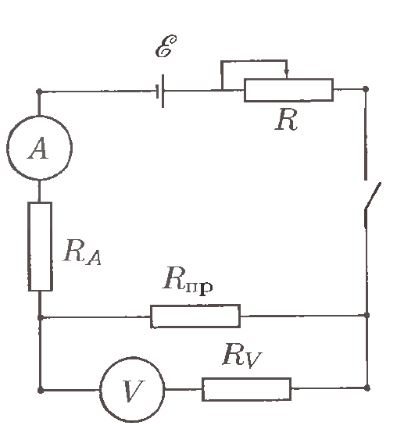
\includegraphics[width = 0.5\linewidth]{1.png}
		\caption{Используемая схема}
		\label{fig:enter-label}
	\end{figure}
	
	Вольтметр верно измеряет падение напряжения на проволоке, а амперметр измеряет сумму токов через проволоку и вольтметр. Поэтому можно записать систему:\\
	\begin{equation*}
		\begin{cases}
			$I_{A} = I + I_{V}$,\\
			$IR = U_{V}$,\\
			$I_{V}R_{V} = U_{V}$
		\end{cases}
	\end{equation*}
	$U_{V}$ - показания вольтметра, $I_{A}$ - показания амперметра\\\\
	Выразив токи $I$ и $I_{V}$ и подставив их в первое уравнение получим\\
	$$R_{\text{1}} = \frac{U_{V}}{I_{A}}= R\frac{R_{V}}{R+R_{V}}$$
	
	\section{Оборудование и экспериментальные погрешности}
	
	\emph{Линейка}: $\Delta_{\text{лин}} = \pm 0.5$ мм (половина цены деления)\\
	\emph{Штангенциркуль}: $\Delta_{\text{шт}} = \pm 0.05$ мм (половина цены деления)\\
	\emph{Микрометр}: $\Delta_{\text{микм}} = \pm 0.01$ мм (маркировка производителя)\\
	\emph{Амперметр}: $\Delta_{\text{А}} = \\
	\emph{Вольтметр}: $\Delta_{\text{V}} = \\
	
	\section{Измерения и обработка данных}
	
	\subsection{Измерение длины проволоки $l$}
	Значения $l$ измерялись с помощью линейки, результаты приведены в Табл. 1
	
	\subsection{Измерение диаметра проволоки $d$}
	Проволока неоднородна, поэтому ее диаметр различен в разных местах. Мы можем измерить его в нескольких местах и усреднить полученные значения.\\\\
	Измерения с помощью штангенциркуля показали одинаковый диаметр проволоки для $N = 12$ измерений, $d_{\text{шт}} = 0.4 \text{мм}$.\\
	\begin{table}[!ht]
		\centering
		\begin{tabular}{|l|l|l|l|l|l|l|l|l|l|l|l|l|}
			\hline
			№ & 1 & 2 & 3 & 4 & 5 & 6 & 7 & 8 & 9 & 10 & 11 & 12 \\ \hline
			$d_{\text{шт}}$, мм & 0.4 & 0.4 & 0.4 & 0.4 & 0.4 & 0.4 & 0.4 & 0.4 & 0.4 & 0.4 & 0.4 & 0.4 \\ \hline
		\end{tabular}
	\end{table}
	Для измерения диаметра был также использован микрометр, который выявил отличия в диаметре проволоки в разных ее местах (см. Табл. 1).
	\begin{table}[!ht]
		\centering
		\begin{tabular}{|l|l|l|l|l|l|l|l|l|l|l|l|l|}
			\hline
			№ & 1 & 2 & 3 & 4 & 5 & 6 & 7 & 8 & 9 & 10 & 11 & 12 \\ \hline
			d, мкм & 380 & 380 & 360 & 390 & 360 & 370 & 350 & 340 & 360 & 380 & 370 & 370 \\ \hline
		\end{tabular}
	\end{table}
	
	\subsection{Вычисление сопротивления проволоки $R$}
	Измерить сопротивление отрезка проволоки $R$ возможно двумя способами
	
	\subsubsection{Метод вычисления $R$ путем анализа ВАХ проволоки}
	Для снятия ВАХ проволоки была собрана схема Рис. 1\\
	ВАХ снималась для трех разных длин проволоки путем постепенного уменьшения напряжения источника. Результаты измерений приведены в Табл. 3
	\\
	
	\begin{table}[!ht]
		\centering
		\begin{tabular}{|l|l|l|l|l|}
			\hline
			№ & Uист, В & Uv, дел & Uv, мВ & Ia, мА \\ \hline
			1 & 3.5 & 148 & 592 & 111.16 \\ \hline
			2 & 3.3 & 137 & 548 & 103.42 \\ \hline
			3 & 3.1 & 130 & 520 & 97.84 \\ \hline
			4 & 2.9 & 121 & 484 & 90.41 \\ \hline
			5 & 2.7 & 115 & 460 & 86.6 \\ \hline
			6 & 2.3 & 98 & 392 & 73.78 \\ \hline
			7 & 1.9 & 80 & 320 & 60.3 \\ \hline
			8 & 1.5 & 64 & 256 & 47.9 \\ \hline
			9 & 1.1 & 36 & 144 & 26.63 \\ \hline
			10 & 0.7 & 23 & 92 & 17.29 \\ \hline
			11 & 0.2 & 3 & 12 & 1.98 \\ \hline
		\end{tabular}
	\end{table}
	
	\subsubsection{Метод прямого измерения $R$ с помощью моста постоянного тока}
	Для измерения $R$ использовался мост постоянного тока Р4833. Для трех $l$ были подобраны такие положения рубильников, при котором стрелка прибора была минимально отклонена от нуля.\\
	Для $l = 20 \text{ см}$ $R = \Omega$;\\
	для $l = 30 \text{ см}$ $R = \Omega$;\\
	для $l = 50 \text{ см}$ $R = \Omega$;\\
	
	
	
	
\end{document}
